\documentclass{article}

\usepackage{hyperref}
\hypersetup{
	colorlinks=true,
	linkcolor=blue,
	urlcolor=cyan,}
\usepackage{booktabs}
\usepackage{textgreek}
\usepackage{amsmath}

%%%%%%%%%%%%%%%%%%%%%%%%%%%%%%%%%%%%%%%%%
% Lachaise Assignment
% Structure Specification File
% Version 1.0 (26/6/2018)
%
% This template originates from:
% http://www.LaTeXTemplates.com
%
% Authors:
% Marion Lachaise & François Févotte
% Vel (vel@LaTeXTemplates.com)
%
% License:
% CC BY-NC-SA 3.0 (http://creativecommons.org/licenses/by-nc-sa/3.0/)
% 
%%%%%%%%%%%%%%%%%%%%%%%%%%%%%%%%%%%%%%%%%

%----------------------------------------------------------------------------------------
%	PACKAGES AND OTHER DOCUMENT CONFIGURATIONS
%----------------------------------------------------------------------------------------

\usepackage{amsmath,amsfonts,stmaryrd,amssymb} % Math packages

\usepackage{enumerate} % Custom item numbers for enumerations

\usepackage[ruled]{algorithm2e} % Algorithms

\usepackage[framemethod=tikz]{mdframed} % Allows defining custom boxed/framed environments

\usepackage{listings} % File listings, with syntax highlighting
\lstset{
	basicstyle=\ttfamily, % Typeset listings in monospace font
}

%----------------------------------------------------------------------------------------
%	DOCUMENT MARGINS
%----------------------------------------------------------------------------------------

\usepackage{geometry} % Required for adjusting page dimensions and margins

\geometry{
	paper=a4paper, % Paper size, change to letterpaper for US letter size
	top=2.5cm, % Top margin
	bottom=3cm, % Bottom margin
	left=2.5cm, % Left margin
	right=2.5cm, % Right margin
	headheight=14pt, % Header height
	footskip=1.5cm, % Space from the bottom margin to the baseline of the footer
	headsep=1.2cm, % Space from the top margin to the baseline of the header
	%showframe, % Uncomment to show how the type block is set on the page
}

%----------------------------------------------------------------------------------------
%	FONTS
%----------------------------------------------------------------------------------------

\usepackage[utf8]{inputenc} % Required for inputting international characters
\usepackage[T1]{fontenc} % Output font encoding for international characters

\usepackage{XCharter} % Use the XCharter fonts

%----------------------------------------------------------------------------------------
%	COMMAND LINE ENVIRONMENT
%----------------------------------------------------------------------------------------

% Usage:
% \begin{commandline}
%	\begin{verbatim}
%		$ ls
%		
%		Applications	Desktop	...
%	\end{verbatim}
% \end{commandline}

\mdfdefinestyle{commandline}{
	leftmargin=10pt,
	rightmargin=10pt,
	innerleftmargin=15pt,
	middlelinecolor=black!50!white,
	middlelinewidth=2pt,
	frametitlerule=false,
	backgroundcolor=black!5!white,
	frametitle={Command Line},
	frametitlefont={\normalfont\sffamily\color{white}\hspace{-1em}},
	frametitlebackgroundcolor=black!50!white,
	nobreak,
}

% Define a custom environment for command-line snapshots
\newenvironment{commandline}{
	\medskip
	\begin{mdframed}[style=commandline]
}{
	\end{mdframed}
	\medskip
}

%----------------------------------------------------------------------------------------
%	FILE CONTENTS ENVIRONMENT
%----------------------------------------------------------------------------------------

% Usage:
% \begin{file}[optional filename, defaults to "File"]
%	File contents, for example, with a listings environment
% \end{file}

\mdfdefinestyle{file}{
	innertopmargin=1.6\baselineskip,
	innerbottommargin=0.8\baselineskip,
	topline=false, bottomline=false,
	leftline=false, rightline=false,
	leftmargin=2cm,
	rightmargin=2cm,
	singleextra={%
		\draw[fill=black!10!white](P)++(0,-1.2em)rectangle(P-|O);
		\node[anchor=north west]
		at(P-|O){\ttfamily\mdfilename};
		%
		\def\l{3em}
		\draw(O-|P)++(-\l,0)--++(\l,\l)--(P)--(P-|O)--(O)--cycle;
		\draw(O-|P)++(-\l,0)--++(0,\l)--++(\l,0);
	},
	nobreak,
}

% Define a custom environment for file contents
\newenvironment{file}[1][File]{ % Set the default filename to "File"
	\medskip
	\newcommand{\mdfilename}{#1}
	\begin{mdframed}[style=file]
}{
	\end{mdframed}
	\medskip
}

%----------------------------------------------------------------------------------------
%	NUMBERED QUESTIONS ENVIRONMENT
%----------------------------------------------------------------------------------------

% Usage:
% \begin{question}[optional title]
%	Question contents
% \end{question}

\mdfdefinestyle{question}{
	innertopmargin=1.2\baselineskip,
	innerbottommargin=0.8\baselineskip,
	roundcorner=5pt,
	nobreak,
	singleextra={%
		\draw(P-|O)node[xshift=1em,anchor=west,fill=white,draw,rounded corners=5pt]{%
		Question \theQuestion\questionTitle};
	},
}

\newcounter{Question} % Stores the current question number that gets iterated with each new question

% Define a custom environment for numbered questions
\newenvironment{question}[1][\unskip]{
	\bigskip
	\stepcounter{Question}
	\newcommand{\questionTitle}{~#1}
	\begin{mdframed}[style=question]
}{
	\end{mdframed}
	\medskip
}

%----------------------------------------------------------------------------------------
%	WARNING TEXT ENVIRONMENT
%----------------------------------------------------------------------------------------

% Usage:
% \begin{warn}[optional title, defaults to "Warning:"]
%	Contents
% \end{warn}

\mdfdefinestyle{warning}{
	topline=false, bottomline=false,
	leftline=false, rightline=false,
	nobreak,
	singleextra={%
		\draw(P-|O)++(-0.5em,0)node(tmp1){};
		\draw(P-|O)++(0.5em,0)node(tmp2){};
		\fill[black,rotate around={45:(P-|O)}](tmp1)rectangle(tmp2);
		\node at(P-|O){\color{white}\scriptsize\bf !};
		\draw[very thick](P-|O)++(0,-1em)--(O);%--(O-|P);
	}
}

% Define a custom environment for warning text
\newenvironment{warn}[1][Warning:]{ % Set the default warning to "Warning:"
	\medskip
	\begin{mdframed}[style=warning]
		\noindent{\textbf{#1}}
}{
	\end{mdframed}
}

%----------------------------------------------------------------------------------------
%	INFORMATION ENVIRONMENT
%----------------------------------------------------------------------------------------

% Usage:
% \begin{info}[optional title, defaults to "Info:"]
% 	contents
% 	\end{info}

\mdfdefinestyle{info}{%
	topline=false, bottomline=false,
	leftline=false, rightline=false,
	nobreak,
	singleextra={%
		\fill[black](P-|O)circle[radius=0.4em];
		\node at(P-|O){\color{white}\scriptsize\bf i};
		\draw[very thick](P-|O)++(0,-0.8em)--(O);%--(O-|P);
	}
}

% Define a custom environment for information
\newenvironment{info}[1][Info:]{ % Set the default title to "Info:"
	\medskip
	\begin{mdframed}[style=info]
		\noindent{\textbf{#1}}
}{
	\end{mdframed}
}
 % Include the file specifying the document structure and custom commands

%----------------------------------------------------------------------------------------
%	ASSIGNMENT INFORMATION
%----------------------------------------------------------------------------------------

\title{EMG Lab 1: Introduction to ELVIS Virtual Instrumentation}
\author{BIOE 385 Bioinstrumentation Laboratory} 
\date{}
%----------------------------------------------------------------------------------------

\begin{document}
\large
\maketitle

\section*{Goals}
\begin{enumerate}
	\item Use NI ELVIS Bode Analyzer to obtain a plot that describes a filter’s response.
	\item Design and build passive filters (low-pass, high-pass, band-pass and band-stop) given a desired cut-off frequency.
	\item Design and build active filters (low-pass, high-pass, band-pass and band-stop) given a desired cut-off frequency.
\end{enumerate}

\section*{Textbook Readings}
Note: these readings will help you with your project.  You are responsible for knowing this information before lab.
\begin{itemize}
	\item 2.31: Decibels
	\item 8.1-7: Operational Amplifiers
	\item 9 (all): Filters
\end{itemize}

\section*{In-lab Assignment}
\subsection*{RC Circuits}

A spring stores mechanical potential energy when it is compressed. Analogously, a capacitor stores electrical energy when opposing charge accumulates on its two conducting surfaces, or plates. Capacitance is defined as the ratio of charge on each plate to the potential difference between them.

$$C = \frac{Q}{V}$$

The SI unit of capacitance is the Farad(F):

$$1\ Farad = \frac{1\ Coulomb}{1\ Volt}$$

Capacitors are referred to as storage elements , because they are capable of storing electrical energy. Incorporating them into electric circuits yields relationships between voltages and currents that can change with time. The most basic configuration of an RC circuit is the circuit given below, commonly referred to as a \textit{low pass filter}.

\begin{figure}[h]
    	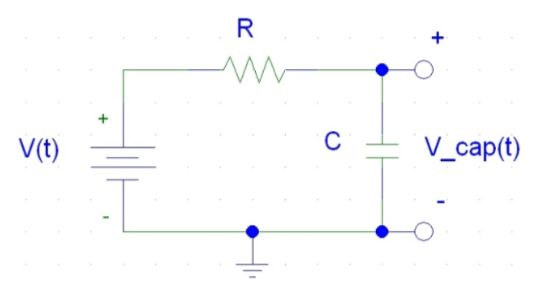
\includegraphics[width=0.5\textwidth]{lab_1_fig_1.jpg}
    	\centering
		\end{figure}

\subsection*{Transient RC Analysis}
We can apply Kirchhoff’s laws to circuits containing capacitors in the same way that we saw for resistors and voltage sources in lecture. Applying Kirchhoff’s voltage law clockwise around the loop, starting at the negative terminal of the battery, yields a first order differential equation describing the charge accumulated on the capacitor as a function of time q(t). The magnitude of current flow is also a function of time:

$$V(t) - I(t)R - V_{cap}(t) = 0$$

$$V(t) - R\frac{dq}{dt} - \frac{q(t)}{C} = 0$$

We would like to describe the voltage across the capacitor as it charges, Vcap(t), so we need to solve for q(t), the charge as a function of time. If we connect the battery at t= 0, then:

$$V(t) = \begin{cases} 0 & t < 0 \\V & t \geq 0 \end{cases}$$

We can solve the differential equation for q(t) by arranging terms containing q and t together on opposite sides and integrating:

$$\int^q_0\frac{dq}{(q-CV)} = -\frac{1}{RC}\int^t_0 dt$$

$$\ln{\Big(\frac{q-CV}{-CV}\Big)} = -\frac{t}{RC}$$

$$q-CV = -CVe^{-\frac{t}{RC}}$$

$$q(t) = CV\Big(1-e^{-\frac{t}{RC}}\Big)$$

$$q(t) = Q\Big(1-e^{-\frac{t}{\tau}}\Big)$$

The time constant, denoted $\tau = RC$, is the length of time necessary for the argument of the exponential term to equal –1. If the voltage is growing, $\tau$ represents the time at which the charge (or voltage) has grown to 63\% of its maximum value.

\subsection*{Charging and Discharging a Capacitor}
Construct the following circuit on the breadboard:

\begin{figure}[h]
    	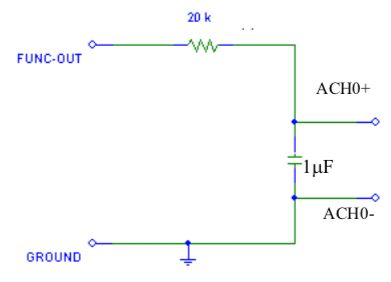
\includegraphics[width=0.5\textwidth]{lab_1_fig_2.jpg}
    	\centering
		\end{figure}

\begin{enumerate}
	\item Connect a 20k\textOmega\ and a 1\textmu F capacitor in series. Apply a signal from the function generator by connecting a wire from your Function Generator (FGEN or FUNC-OUT) to the resistor terminal. Ground the other capacitor terminal. What is the time constant of this circuit? Show your calculations.
	\item Connect the terminals of the capacitor to AI 0+ and AI 0- of the virtual oscilloscope using a wire.
	\item On the computer, open the Virtual Instrument Function Generator . Make sure that the switch on the front panel of the ELVIS unit is NOT on “Manual”. Select a square waveform with the following parameters: Frequency: 5 Hz, Amplitude: 4.0 V\textsubscript{p-p}, DC Offset: 2.0 V.
	\item Now open the Oscilloscope virtual instrument. Stabilize the signal using a trigger (recommended settings: Digital, SYNC). You should see a stable filtered signal on the screen.
	\item Adjust your scale and use the cursors in the oscilloscope screen to calculate the time it takes for the capacitor voltage to go from its minimal value to 95\% of its maximal value. Divide this estimate by 3 to get a measure of the time constant.
	\item Show the instructor or a TA your results.
\end{enumerate}

\subsection*{Passive Filters}
\begin{figure}[h]
    	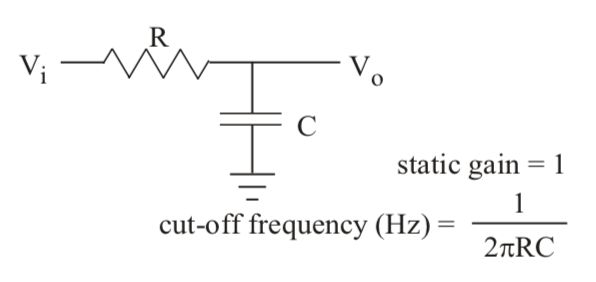
\includegraphics[width=0.5\textwidth]{lab_1_fig_3.jpg}
    	\centering
		\end{figure}
		
\begin{enumerate}
	\item A passive low-pass filter can be constructed with a resistor and capacitor alone as shown in the figure above. Build one using a 10k\textOmega\ resistor and a 0.1\textmu F capacitor. Starting with a frequency of about 10 Hz, input a 1 V sine wave (zero offset) into the low-pass filter circuit. Calculate values for the cut-off frequency and the time constant.
	\item Test the filter to make sure that it works. We expect that it will allow frequencies below the cut-off frequency to "pass", while attenuating higher frequency signals. Viewing both signals on the oscilloscope, slowly increase the frequency of the input signal. What happens to the output signal?
	\item Create a second order filter with the same cutoff frequencies as in the previous exercise. Run the Bode Analyzer and Log your data. Do the magnitude ratio and phase difference between the input and output behave as you would expect?
	\item Create a third order filter with the same cutoff frequencies as in the previous exercise. Run the Bode Analyzer and Log your data.
\end{enumerate}

\subsection*{Active Filters}
\begin{enumerate}
	\item The filters shown below are active filters - since they use an op-amp, they can have a static gain greater than one. The configuration in (a) is a non-inverting first-order active low-pass filter, and (b) is an inverting first-order active low-pass filter. The filter is called first-order because its dynamics are modeled by a first-order differential equation. Calculate values for the cut-off frequency and the time constant of one active low pass filter with R1= 10k\textOmega, C1= 0.1\textmu F and a gain of 1.
	\begin{figure}[h]
    	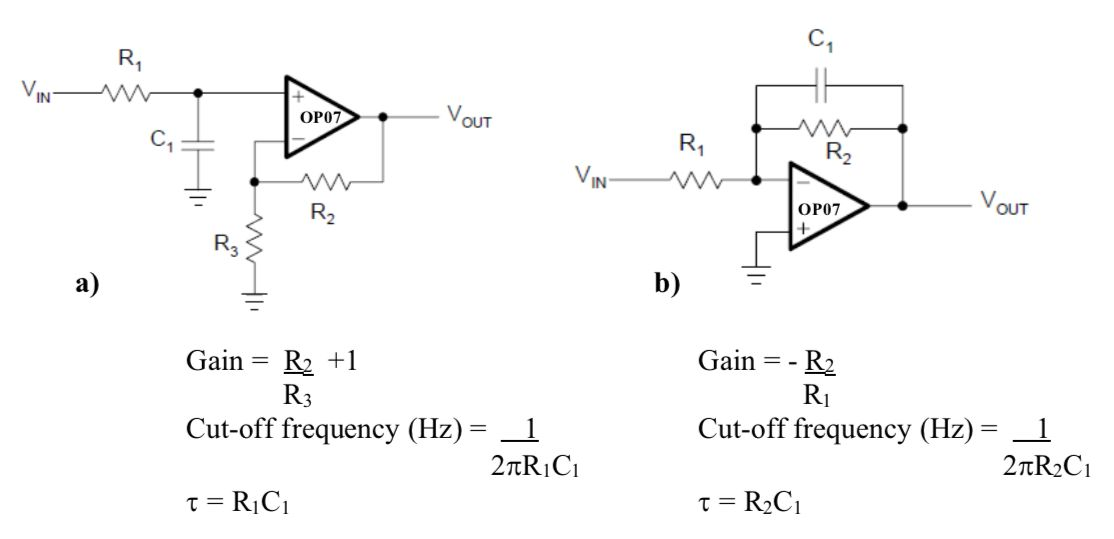
\includegraphics[width=0.9\textwidth]{lab_1_fig_4.jpg}
    	\centering
		\end{figure}
	\item Implement one of the first-order filters shown in Figure 2. The next step is to test the filter to make sure that it works. We expect that it will allow frequencies below the cut-off frequency to "pass", while attenuating higher frequency signals. Starting with a frequency of about 10 Hz, input a 1 V sine wave (zero offset) into the low-pass filter circuit. Viewing both signals on the oscilloscope, slowly increase the frequency of the input signal. What happens to the output signal? Run the Bode Analyzer on this circuit. Save the data in a log as well.
	\item Create an active High-Pass Filter with the same cut-off frequencies as in 1.
	\item Show all the bode plots from the filters you have built so far today on one Excel file. Label them well. (i.e. resistor values, filter type, desired filter cut off frequency). Write a statement comparing and contrasting the output of the different filters.
\end{enumerate}

\subsection*{Bandpass Filters}
\begin{enumerate}
	\item Now design and build a band-pass filter. Select your 2 cut-off frequencies. You may use either active or passive filters. Draw your circuit, report your desired cut-off frequencies and justify your choices in resistors and capacitors values.
	\item Create a Bode plot of the output from your filter. Demonstrate this to the instructor or a TA.
\end{enumerate}
\end{document}
